\section{Isometrie}
$A: \mathbb{R}^{2} \rightarrow \mathbb{R}^{2}$\\
$\Vert Av \Vert = \Vert v \Vert$\\
\qquad\\
 \begin{tabular}{c|c}
 	Drehung & Spiegelung \\ \hline
  	$det(A) = 1$ & $det(A) = 1$ \\ 
  	$R_{c,s}=\begin{pmatrix} c & -s \\ s & c \end{pmatrix}$ & $S_{c,s} = \begin{pmatrix} c & s \\ s & -c \end{pmatrix}$\\
 	$c^{2}+s^{2} = 1$ & $c^{2}+s^{2} = 1$\\
 \end{tabular}
 %
 \begin{figure}[H]
 \centering
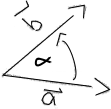
\includegraphics[width=0.1\textwidth]{mainmatter/chapter1/pics/bewegung2.png}
\end{figure}
 %
 \subsubsection{Definition (Winkel):}
 Sind $a,b \in \mathbb{R}^{2}\diagdown \{0\}$ Vektoren dann heißt die eindeutige Drehung $\alpha =R_{c,s}$ mit $\alpha(a)=\lambda\cdot b, \, \lambda \in \mathbb{R}_{\geq 0}$ der Winkel zwischen $a$ und $b$, und wir schreiben $\alpha := < (a,b)$\\
 Die Summe $\alpha + \beta$ zweier Winkel $\alpha$ und $\beta$ definieren wir als $\alpha + \beta := \alpha \circ \beta$ (beachte $\alpha + \beta = \beta + \alpha$)\\
 Das Negative eines Winkels $\alpha$ definieren wir als $-\alpha := \alpha ^{-1}$ d.h. ist $\alpha = R_{cs} \Rightarrow \alpha^{-1} = R_{c,-s}$ Sind $A,B,C \in \mathbb{R}^{2}$ Punkte, dann definieren wir den Winkel an Punkt $A$ des Tripels $(ABC)$ als < $(B,A,C) := < (B-A,C-A)$. 
 %
 %
 %
 \subsubsection{Definition (Winkelhalbierende):}
 Ist $\alpha$ ein Winkel, dann existiert ein Winkel $\beta$ mit $\beta + \beta = \alpha$. Dieser heißt der halbe Winkel zu $\alpha$ oder auch die Winkelhalbierende zu $\alpha$.
 %
 %
 %
 \subsubsection{Satz:}
 Ist $\alpha = R_{c,s}$ so kann man $\beta = R_{t,u}$ wählen mit \\
 $t = \pm \sqrt{\frac{1}{2}(1+c)}, \, u=\sqrt{\frac{1}{2}(1-c)}$ wobei $"`+"' \Leftrightarrow s \geq 0$. 
 %
 %
 %
 \subsubsection{Beweis:}
 Nehmen wir an, dass $\alpha = 2 \beta$ mit $\alpha = \begin{pmatrix} c & -s \\ s & c \end{pmatrix}, \, \beta = \begin{pmatrix} t & -u \\ u & t \end{pmatrix}$\\
 $\Rightarrow \begin{pmatrix} c & -s \\ s & c \end{pmatrix} = \begin{pmatrix} t & -u \\ u & t \end{pmatrix} \begin{pmatrix} t & -u \\ u & t \end{pmatrix} = \begin{pmatrix} t^{2}-u^{2} & -2tu \\ 2tu & t^{2}-u^{2} \end{pmatrix}$\\
 \qquad\\
 Es gilt also $c=t^{2}-u^{2}, \, s=2tu$\\ 
 \qquad\\
$
\begin{array}{rcrcr}
c \cdot 4t^{2} &=& 4t^{4} &-& 4u^{2}t^{2}\\
 &=& 4t^{4} &-&  s^{2}\\
 &=& 4t^{4} &-& (1-c^{2})
\end{array} 
$\\
\qquad\\
\qquad\\
$ \Rightarrow t^{4} - c\cdot t^{2} - \frac{1}{4}(1-c^{2})=0$\\
$\mathop{\Rightarrow}\limits^{\text{pq}}t^{2} = \frac{c}{2} \pm \sqrt{\frac{c^{2}}{4}+\frac{1}{4}(1-c^{2})} = \frac{c}{2} \pm \frac{1}{2}=\frac{1}{2}(c\pm 1) \geq 0$\\
\qquad\\
Wir wissen $1=c^{2}+s^{2}\geq 0 \Rightarrow  -1 \leq c \leq 1$\\
wegen $1=t^{2}+u^{2}\Rightarrow 0 \leq t^{2}\leq 1$\\
Würden oben ein "`-"' stehen, wäre $t^{2} < 0$ für $c<0 \lightning$\\
$\Rightarrow t^{2} = \frac{1}{2}(c+1) \Rightarrow t = \pm \sqrt{\frac{1}{2}(c+1)}$\\
Analog folgt $u=\sqrt{\frac{1}{2}(1-c)}$ \\
$t^{2}-u^{2} = \frac{1}{2}(c+1)-\frac{1}{2}(1-c)=\frac{1}{2}c + \frac{1}{2}c = c$\\
$2tu=2\cdot(\pm\sqrt{\frac{1}{2}(1+c)\cdot\frac{1}{2}(1-c)} = \pm 2 \sqrt{\frac{1}{4}\mathop{\underbrace{(1-c^{2})}}\limits_{s^{2}}} = \pm \sqrt{s^{2}} = \pm \vert s \vert \mathop{=}\limits^{\text{!}} s$\\
Die letzte Gleichheit gilt genau dann, wenn $\pm$ das Vorzeichen von $s$ ist (d.h. "`+"' $\Leftrightarrow \, s \geq 0$).\\
\qquad\\
Wir messen Winkel, indem wir der Drehung $\begin{pmatrix} -1 & 0 \\ 0 & -1 \end{pmatrix}$ den Wert 180$^{\circ}$ oder $\pi$ zuweisen.\\
Durch das Halbieren und Addieren von Winkeln können wir jeden Winkel eine Zahl $0^{\circ} \leq x \leq 360^{\circ}$ zuordnen, die wir das Winkelmaß nennen. \\
z.B. $\frac{1}{3} = \sum\limits^{\infty}_{n=1} \frac{1}{4^{n}}$\\
Tatsächlich lässt sich jede Zahl $ 0 \leq x \leq 360 $ schreiben als $360^{\circ} \cdot  \sum\limits^{\infty}_{n=1}a_{n}\frac{1}{2^{n}}, \qquad a_{n}\in  \mathbb{N}_{0}$ \\
Was ist der halbe Winkel zu $\begin{pmatrix} -1 & 0 \\ 0 & -1 \end{pmatrix}$ ?\\
$R_{t,u}$ mit $t = \pm \sqrt{\frac{1}{2}(1+c)} = 0$\\
$ u = \sqrt{\frac{1}{2}(1-c)} = 1$ d.h. $R_{t,u} = \begin{pmatrix} 0 & 1 \\ 1 & 0 \end{pmatrix} \mathrel{\widehat{=}} 90^{\circ} = \mathop{\alpha}\limits^{\text{\RM{2}}}$
%
%
%
\subsubsection{Satz (Winkelsumme im Dreiecke):}
 \begin{figure}[H]
 \centering
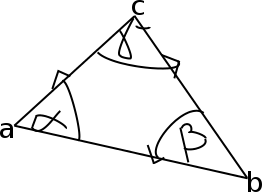
\includegraphics[width=0.2\textwidth]{mainmatter/chapter1/pics/winkelsumme.png}
\end{figure}
Es sei $a,b,c$ ein Dreieck (d.h. $a,b,c$ sind Punkte) und $\alpha := \measuredangle ( b,a,c), \, \beta := \measuredangle(c,b,a), \, \gamma := \measuredangle (a,c,b)$\\
Dann gilt $\alpha + \beta + \gamma = 180^{\circ} (=\pi)$
%
%
%
\subsubsection{Beweis:}
$\alpha(b-a)=\lambda(c-a), \, \lambda \in \mathbb{R}_{>0}$\\
$\beta(c-b)=\mu(a-b), \, \mu \in \mathbb{R}_{>0}$\\
$\gamma(a-c)= r(b-c), \, r \in \mathbb{R}_{>0}$\\
\qquad\\
$
\begin{array}{rcr}
(\alpha + \beta + \gamma)(a-c) &\mathop{=}\limits^{\text{Definition}}& \alpha \circ \beta \circ \gamma(a-c)\\
 &=&  \alpha (\beta(\gamma(a-c)))\\
 &=& \alpha(\beta(r(b-c)))\\
 &=& \alpha (\beta(-r(c-b)))\\
 &=& -r \cdot \alpha(\beta(c-b))\\
 &=& -r\cdot \alpha(\mu(a-b))\\
 &=& \mu \cdot r \cdot \alpha (b-a)\\
 &=& -\alpha \mu r (a-c)
\end{array} 
$\\
Da $\alpha + \beta + \gamma$ wieder eine Drehung ist, gilt $\Vert a-c\Vert = \Vert (\alpha + \beta + \gamma)(a-c)\Vert=\vert\lambda \mu r\vert \cdot \Vert (a-c)\Vert \Rightarrow \vert \lambda \mu r\vert=1$\\
Da $\alpha, \mu, r > 0 \Rightarrow \lambda\mu r = 1$\\
Somit gilt \\
($\alpha+\beta+\gamma)(a-c)=-\lambda \mu r (a-c) = -1(a-c)=\begin{pmatrix} -1 & 0 \\ 0 & -1\end{pmatrix}(a-c) \Rightarrow \alpha + \beta + \gamma=180^{\circ} \rightarrow$ Winkelsumme $\square$
%
%
%
\subsubsection{Korollar:}
In einem Viereck ist die Summe der Innenwinkel $360^{\circ}$
%
%
%
\subsubsection{Beweis:}
Zerlege das Viereck durch Verbinden zweier nicht verbundenen Ecken in 2 Dreiecke:
%
 \begin{figure}[H]
 \centering
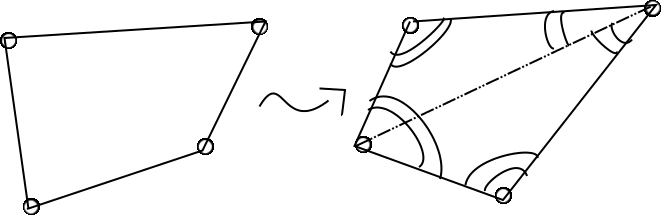
\includegraphics[width=0.3\textwidth]{mainmatter/chapter1/pics/winkeladd.png}
\end{figure}
%
\subsubsection{Satz(Gleichschenklige Dreiecke):}
Sei $a,b,c$ ein gleichschenkliges Dreieck, d.h. $\Vert a-c \Vert = \Vert b-c \Vert$, dann gilt $\measuredangle (b,a,c) = \measuredangle (c,b,a)$
%
 \begin{figure}[H]
 \centering
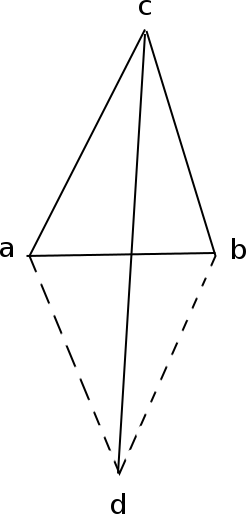
\includegraphics[width=0.1\textwidth]{mainmatter/chapter1/pics/para.png}
\end{figure}
%
\subsubsection{Beweis:}
o.E. gilt $c=0$\\
Dann gilt also $a-c=a, \, b-c=b$.\\
Es sei $d:=a+b$. \\
\qquad\\
Behauptung:\\
 $a+b\perp a-b$\\
 \qquad\\
Beweis:\\
$<a+b,a-b>=<a,a>+<b,a>-<a,b>-<b,b>=\Vert a \Vert^{2}-\Vert b \Vert^{2} = 0$ nach Voraussetzung $\Vert a \Vert = \Vert b \Vert$\\
%
 \begin{figure}[H]
 \centering
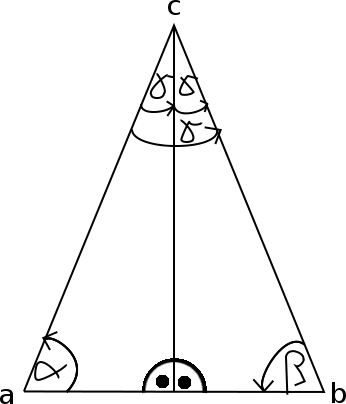
\includegraphics[width=0.15\textwidth]{mainmatter/chapter1/pics/gleichbeweis.png}
\end{figure}
%
$m:=\frac{1}{2}(a+b)$\\
$\alpha + \gamma_{1} - \frac{\pi}{2}=\pi \Rightarrow \alpha + \gamma_{1} = \frac{\pi}{2}$\\
$\beta+\gamma_{2}+\frac{\pi}{2}=\pi\Rightarrow\beta+\gamma_{2}=\frac{\pi}{2}$\\
Wir zeigen $\gamma_{1}=\gamma_{2}$ indem wir zeigen, dass $m$ auf der Winkelhalbierenden von $\gamma$ liegt. \\
$R(\vec{a})=\lambda b$\\
$R_{\gamma}=\begin{pmatrix} c & -s \\ s & c \end{pmatrix}$\\
$R_{\frac{\gamma}{2}}=\begin{pmatrix} \sqrt{\frac{1}{2} (1+c)} & - \sqrt{\frac{1}{2}(1-c)} \\ \sqrt{\frac{1}{2}(1-c)} & \sqrt{\frac{1}{2}(1+c)}\end{pmatrix} \qquad u=\begin{pmatrix} a_{1} \\ a_{2} \end{pmatrix}$\\
$\lambda :=\sqrt{\frac{1}{2}(1+c)}$\\
$\lambda \cdot R_{\frac{\gamma}{2}} \cdot \vec{u} = \begin{pmatrix} \frac{1}{2} (1+c)a_{1} -\frac{1}{2}\sqrt{1-c^{2}}a_{2} \\ \frac{1}{2}\sqrt{1-c^{2}}a_{1} + \frac{1}{2}(1+c)a_{2}\end{pmatrix}$\\
$= \frac{1}{2}(\begin{pmatrix}a_{1} \\ a_{2} \end{pmatrix} + R_{\gamma} \begin{pmatrix} a_{1} \\ a_{2} \end{pmatrix} ) = \frac{1}{2}(\vec{a}+\vec{b}=\vec{m}$\\
$\vec{m}$ liegt also auf der Winkelhalbierenden von $\gamma \Rightarrow \gamma_{1} = \gamma_{2} = \frac{\gamma}{2}$